\section*{Решения и комментарии}

\subsubsection*{Отгадать цвет шляп}

Как мы предупреждали, случай трёх игроков помогает найти решение.
Как минимум, он даёт возможность убедиться, что $50\%$ можно улучшить.
Однако получить отсюда общий случай непросто.

Каждого из трёх игроков, следует проинструктировать молчать если он видит шляпы разных цветов,
а если обе шляпы одного цвета, то называть цвет который он \emph{не видит}.
В случае если есть шляпы обоих цветов (а это шесть из восьми случаев) один назовёт правильный цвет, а два других промолчат.
В результате игроки выигрывают с вероятностью $75\%$.

Заметим, что в плохих случаях, когда все шляпы одного цвета, \emph{все три} игрока называют неправильный цвет.
То есть данный протокол упаковывает 6 неправильных ответов в две конфигурации, и это имеет решающее значение.
Ведь в среднем по всем конфигурациям, ровно половина угадываний должна быть верной, поэтому чтобы выиграть следует экономно использовать правильные угадывания, а неправильные паковать вместе.
Протокол для трёх игроков делает это наилучшим образом, и значит он является оптимальным.

Для $n$ игроков, было бы идеально сделать тот же самое,
то есть построить два типа конфигураций: «хорошие», где ровно один угадывает правильно и «плохие», в которых угадывают все и все неправильно.
В этом случае хороших конфигураций будет в $n$ раз больше плохих,
что даст неплохую вероятность выигрыша равную $n/(n+1)$.

Такую оптимальную вероятность возможно достичь только если число всех конфигураций, $2^n$, делится на $n+1$;
то есть, если $n$ равно степени двойки без единицы.
Удивительным образом это условие также является достаточным.

Ключ к протоколу состоит в разбиении конфигураций на плохие и хорошие так, что любая хорошая \emph{соседствовала} ровно с одной плохой (две конфигурации соседствуют если одну можно получить из другой поменяв цвет одной шляпы).
И такой способ есть!

Пусть $n=2^k-1$.
Пронумеруем игроков $k$-значным не нулевым кодом в двоичной системе.
(Например, если $n=15$, то игроки нумеруются $0001,0010,0011,\dots,1110,1111$.)
Эти коды будем складывать как ним-числа%
\footnote{Названные так из-за их игры ним.
На сколько нам известно этот неожиданный термин появляется впервые на с. 43 в «Winning Ways».}, то есть без учёта переноса разрядов;
например $1011 + 1101 =0110$ и ним-сумма любого кода с собой равна $0000$.

Плохими конфигурациями будут те, для которых ним-сумма кодов всех игроков с красными шляпами равна $0000$.
Стратегия состоит в следующем:
каждый игрок считает ним-сумму кодов всех кого видит в красных шляпах.
Если ним-сумма равна $0000$, то он говорит, что у него красная шляпа.
Если же ним-сумма равна его коду, он говорит, что у него синяя шляпа.
В остальных случаях он молчит.

А почему это работает?
Предположим, что ним-сумма кодов \emph{всех} игроков с красными шляпами равна $0000$.
Тогда для каждого игрока с синей шляпой посчитанная им ним-сумма будет $0000$ и он скажет, что у него красная шляпа;
ним-сумма посчитанная каждым игроком с красной шляпой будет его кодом и он скажет что у него синяя шляпа.
То есть каждый назовёт цвет и каждый сделает это неправильно --- ровно то, что мы хотели!

Теперь  предположим, что эта ним-сумма равна чему-то другому, например $0101$.
Тогда цвет назовёт единственный игрок с кодом  $0101$ и назовёт он его \emph{правильно}.

Ним-сумма равна $0000$ с вероятностью $1/16$ (поскольку имеется 16 различных ним-сумм).
Значит, вероятность выигрыша составит $15/16$;
в общем случае она равна $1-2^{-k}$.
Полезно проверить, что в случае $k=2$ мы получим наше решение для трёх игроков.

Если $n$ не степень двойки без единицы, то самое простое найти наибольшее $m<n$ вида $2^k-1$.
Эти $m$ игроков следуют описанной стратегии, а все остальные молчат независимо от того, что они видят.
В худшем случае (если $n=2^k-2$ при некотором $k$) вероятность выигрыша равна $(n/2)/((n/2)-1)$.
Вообще говоря, такая стратегия не самая лучшая;
при $n=4$ невозможно улучшить $75\%$, но при $n=5$ (как указал Элвин Берлекэмп) можно добиться вероятности $25/32>78\%$.
В общем случае, наилучшая стратегия неизвестна.
\heart

Построенное нами множество плохих конфигураций не только красиво но и полезно.
Оно называется кодом Хэмминга и является примером идеального самокорректирующегося кода.
Представьте, что вам надо посылать несколько битов информацию по не очень надёжному каналу, который иногда переворачивает бит.
Сгруппируйте биты в строчки по 11 в каждой.
Существует $2^{15}/16\z=2^{11}$ красносиних строк длины 15 с ним-суммой $0000$;
их можно записать двоичным кодом (например код $101010101010101$ значит, что все нечётные шляпы красные).
Эти 15-значные строки будут называться «допустимыми».
Поскольку число допустимых строк равно $2^{11}$, можно выбрать одну для каждой из 11-значных строк.
Простейший способ это сделать --- выбросить последние 4 бита из 15-значной строки.

Чтобы послать строку из 11 битов вы посылаете единственную соответственную ей допустимую строку из 15 битов.
Вы проигрываете в скорости, но взамен получаете надёжность.
Действительно, если один из битов по ошибке перевернулся, то получающая сторона сможет узнать номер этого бита и перевернуть его назад!

Как? А надо взять ним-сумму кодов красных битов (тех что соответствуют единицам) в полученной 15-значной строке и удостоверится, что она равна $0000$.
Пусть нет, скажем она равна $0101$,
тогда какой-то бит перевернулся;
если это случилось только раз, то это должен быть пятый бит.
Значит, следует перевернуть пятый бит и сверится с системой кодов чтобы понять какая 11-значная строка соответствует полученной 15-значной.
Результат будет верен, если только не случилось нескольких переворотов зараз.

\medskip

Эта задача (в несколько другой формулировке) и её решение рассматривалась Тоддом Эбертом (сейчас в Калифорнийском университете в Ирвайне) в его диссертации защищённой в 1998 в Калифорнийском университете в Санта-Барбаре.
Решение с кодом Хэмминга было предложено несколько лет до этого Стивеном Рудичем из Университета Карнеги — Меллона  для похожей задачи про выборы.

\subsection*{15 битов и шпионка}

Поскольку шпионка может произвести всего 16 действий (изменить какой-то бит или никакого), то она \emph{в принципе} может передавать четыре бита информации ежедневно.
Но как?

Ответить на это просто, если воспользоваться ним-суммами из предыдущего решения.
Шпионка и её центр присваивают $k$-тому биту 4-значный код, соответствующий числу $k$, а «сообщение» определяется как ним-сумма кодов с единицами в передаче на радио.

Утверждение состоит в том, что шпионка может передать любое из 16 возможных сообщений по её желанию,
достигая таким образом, четырёх битов информации.
Предположим, она желает послать код $n$, а ним-сумма кодов с единицей в намеченной передаче равна $m\ne n$.
Тогда ей следует поменять бит номером равным ним-сумме $m+n$.
Не имеет значения, был ли этот бит 0 или 1, так как ним-сумма равна ним-разности.
\heart

\medskip

Я узнал эту задачу от Ласло Ловаса из Microsoft Research, который не смог с уверенностью назвать её источник.

\subsubsection*{Углы в пространстве}

Мне дали эту задачу при собеседовании в Массачусетском технологическом институте, и я на ней засыпался.
Кажется, что $2^n$ вершин куба дают наибольшее число точек в $n$-мерном пространстве без тупого угла.
Но как это доказать?
Оказывается этот вопрос был сформулирован Палом Эрдёшем и Виктором Кли и решён Людвигом Данцером и Бранко Грюнбаумом. %реф

\medskip

Пусть $x_1,\dots,x_k$ это различные точки (векторы) в $\mathbb{R}^n$, и пусть $P$ --- их выпуклая оболочка.
Можно предположить, что $P$ имеет объём 1;
этого можно добиться уменьшая размерность пространства до размерности $P$, а затем подобрав подходящий масштаб.
Можно также предположить, что $x_1$ является началом координат (нуль-вектором).
Если эти точки не образуют тупых углов, то для каждого $i>1$, внутренность сдвига $P+x_i$ не перекрывается с внутренностью $P$;
это верно поскольку плоскость через $x_i$, перпендикулярная вектору $x_i$, разделяет эти два многогранника.

Кроме того, внутренности $P+x_i$ и $P+x_j$ также не перекрываются при $i\ne j$;
они разделяются плоскостью через $x_i+x_j$ перпендикулярной к $x_i-x_j$.
Отсюда делаем вывод, что объём объединения $P+x_i$ для $1 \le i \le k$ равен $k$.
Однако все эти многогранники лежат внутри удвоенного многогранника $2P = P+P$, объём которого равен $2^n$. Следовательно, $k \le 2^n$, что и требовалось!
\heart

\subsubsection*{Два монаха на горе}

Давайте разделим каждый путь на монотонные «отрезки», в пределах которых путь всегда восходящий, или всегда нисходящий.
\footnote{Естественно предположить, что существует только конечное число монотонных отрезков, ведь нету смысла рассматривать отрезки существенно короче чем шаг монаха.
Однако если этого не предполагать, то ответ в задаче окажется другим.
%It's reasonable to assume there are only finitely many monotonic segments; it doesn't make sense for a segment to bemuch shorter than a monk's step size. However, if we do not assume that, then the answer to the puzzle will be different.
}
(Отрезки идущие по одному уровню не вызывают проблем, так как один монах может стоять и ждать пока другой проходит такой отрезок).
Можно предположить, что каждый такой отрезок является прямым восхождением или спуском, так как мы можем заставить монахов варьировать скорости так, чтобы их скорость восхождения или спуска была постоянной на любом отрезке.

Пусть ось $X$ на плоскости соответствуют позиции на тропе первого монаха, а ось $Y$ --- позиции второго монаха.
Отметим все точки плоскости для которых оба монаха находятся на одной высоте;
полученный график будет включать в себя начало координат (это начало обоих путей) и вершину (концы обоих путей, можно считать, что это точка (1,1)).
Наша цель состоит в том, чтобы найти путь вдоль построенного графика от (0,0) до (1,1);
монахи смогут медленно проследовать по этому пути, так что ни одному из них не придётся идти быстрее, чем он может.

Любые два отрезка --- по одному от каждого пути --- которые имеют некоторую общую высоту, появляются на участке в виде отрезка, возможно нулевой длины.
Если рассматривать в качестве вершины любую точку, которая соответствует конечной точке такого отрезка (для одного или двух монахов), то график становится графом (в комбинаторном смысле);
простая проверка случаев показывает, что, за все вершины кроме (0,0) и (1,1) являются концами 0, 2 или 4 рёбер.

Если мы начинаем прогулку по графу из (0,0), то нету места в котором можно было бы застрять или быть вынужденным повторять путь, кроме вершины (1,1).
Значит, удастся добраться до (1,1), и любой такой маршрут даст успешную стратегию монахам.
\heart

На рисунке показаны четыре возможных варианта, при этом путь одного монаха показан сплошной линией, а другого пунктирной.
Ниже каждого варианта находится соответствующий график.
Заметим, что, как например в последнем случае, график может иметь участки, к которым у монахов нет доступа (без нарушения равенства высот).

\begin{figure}[h!]
\centering
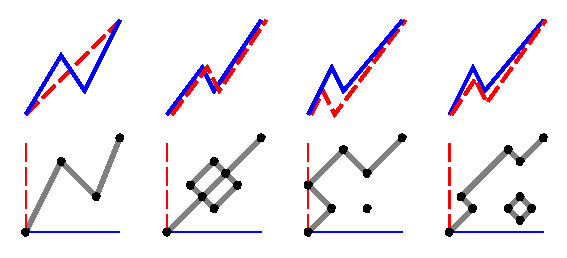
\includegraphics[scale=0.9]{Figs/Toughies/monks}
\end{figure} 

Эту задачу мне показал Юлий Барышников из Лабораторий Белла.

\subsubsection*{Сумма под контролем}

Эта задача возникла «из реальной жизни», или, по крайней мере, из серьёзной задачи про волоконно-оптическую связь.\footnote{A. Schrijver, P. D. Seymour, P. Winkler, ``The Ring Loading Problem''. \emph{SIAM Review} Vol. 41, \#4 (Dec. 1999), 777--791.}
Гипотеза была обнародована, но не было найдено ни доказательств или контрпримеров.
Наконец автор этих строк нашёл доказательство приведённое ниже, которое ещё и оказалось довольно простым!

\medskip

Задача состоит в том, чтобы выбрать знаки в последовательности чисел из отрезка $[0,1]$ так, чтобы сумма была под контролем даже если обратить знак у любого хвоста последовательности.
Первое наблюдение состоит в том, что можно управлять всеми начальными суммами жадным алгоритмом, то есть ставить $y_k=x_k$, если $\sum_{i=1}^{k-1}y_i \le 0$ и $y_k=-x_k$ в противном случае.

Это гарантирует, что $\left|\sum_{i=1}^{k}y_i\right| \le 1$ для любого $k$ и значит
\begin{align*}
\left|\sum_{i=1}^{k}y_i-\sum_{i=k+1}^{n}y_i\right|&=\left|2\sum_{i=1}^{k}y_i-\sum_{i=1}^{n}y_i\right|\le
\\
&\le2\left|\sum_{i=1}^{k}y_i\right|-\left|\sum_{i=1}^{n}y_i\right|\le3.
\end{align*}
Это близко к тому, что нам надо, но оказывается, что любой алгоритм который не заглядывает вперёд, не может улучшить 3 до~2.
Чтобы это увидеть, представьте, что последовательность начинается как
1, 0,99, 1, 0,99, 1, 0,99, и так сто раз, но внезапно заканчивается некоторым числом $z$.
В этом случае знаки должны чередоваться каждый раз кроме одного момента, и чтобы узнать этот момент, необходимо знать $z$.

Однако заметим, что в описанном выше жадном алгоритме требуется знание «пустой суммы», чтобы выбрать первый знак.
Обычно мы считаем, что эта сумма равна 0, но давайте объявим её равной $w$.
Тогда, для фиксированного $w\in [-1,1]$, знаки $y_k$ определяются индуктивно как $y_k=x_k$ если $w+\sum_{i=1}^{k-1}y_i \le 0$, а иначе $y_k=-x_k$.
В этом случае $w+\sum_{i=1}^{k}y_i \in[-1,1]$ для любого $k$.
Рассмотрим функцию $f(w) \mathop{{:}{=}} w+\sum_{i=1}^ny_i$.

Предположим, что $f(w)=-w$.
Тогда
\begin{align*}
&\phantom{=}\sum_{i=1}^{k}y_i-\sum_{i=k+1}^{n}y_i=
\\
&=2\sum_{i=1}^{k}y_i-\sum_{i=1}^{n}y_i=
\\
&=2\left(w+\sum_{i=1}^{k}y_i\right)-\left(w+\sum_{i=1}^{n}y_i\right)-w=
\\
&=2\left(w+\sum_{i=1}^{k}y_i\right)\in[-2,2],
\end{align*}
что и требуется.

Поскольку  $f(-1)+(-1)<0 <f(1)+ 1$, существование $w$, для которого $f(w)=-w$ следовало бы из теоремы о промежуточном значении, если бы $f$ была непрерывна.
Конечно же, это не так; всякий раз, когда частичная сумма проходит через 0, некоторые знаки меняются и $f(w)$ может совершить скачёк.
(Заметим, что $f$ непрерывна слева, поскольку мы выбираем плюс при нулевой частичной сумме.)
Однако \emph{абсолютное значение} $f$ является непрерывным.

Сначала следует отметить, что, если частичные суммы не равны $0$, то производная $f'(w)$ равна 1.
С другой стороны, предположим, что $w=w_0$ таково, что одна или более частичных сумм равна нулю.
Пусть $k > 0$ будет минимальным для которого $w+\sum_{i=1}^{k}y_i\z=0$.
Тогда для достаточно малых $\varepsilon>0$,
знаки $y_j$ и $w+\sum_{i=1}^{j}y_i$ при $j>k$ оборачиваются, при переходе от $w=w_0$ к $w=w_0+\varepsilon$.
Взяв $j = m$, получаем, что $\lim_{w\to w_0^+}f(w)\z=-f(w_0)$.

То есть, если при $w=w_0$ любая из частичных сумм обнуляется, то $\lim_{w\to w_0^+}f(w)\z=-f(w_0)$, таким образом, функция $g$, определяемая как $g(w) =|f(w)|$ будет непрерывной и иметь производную $\pm1$ везде кроме конечного числа точек.
Граф $g$ представляет собой зигзаг с производной $1$ при $g(w)=f(w)$ и $-1$, при $g(w)=-f(w)$.

Если определить функцию $h$ как $h (w) = -w$, то граф $h$ будет отрезком с угловым коэффициентом $-1$ и концами в $(-1,1)$ и $(1,-1)$;
этот отрезок обязан пересекать граф $g$.
Более того, он либо пересекает его в точке, где $g'(w) = 1$, либо совпадает с отрезком графа $g$ с угловым коэффициентом $-1$, в последнем случае самая левая точка отрезка также лежит и на графике $f$.
В обоих случаях, мы получаем точку $w$, в которой $-w = g (w) = f (w)$. \heart

\subsubsection*{Двухлампавая комната}

Эта головоломка является частью серьёзной задачи в распределённых вычислениях.%
\footnote{Больше об этом вопросе можно прочитать в статье M. J. Fischer, S. Moran, S. Rudich, and G. Taubenfeld, ``The Wakeup Problem''. \emph{Proc. 22nd Symp. on the Theory of Computing}, Baltimore, Maryland, May 1990.}
Решение, приведённое ниже, данное Стивеном Рудичем из Университета Карнеги --- Меллона, известно как «протокол с качелями»\footnote{англ. \emph{see-saw protocol}.}.

\medskip

Для понимания этого протокола, удобно думать об одном из переключателей как о «переключателе с камушком», в нём либо лежит камушек либо он пуст, а о другом --- как о качелях, у доски качелей может быть опущен либо правый либо  левый конец (противоположный конец доски должен быть при этом поднят).
Каждый заключённый начинает с двумя виртуальными камушками.

При первом допросе заключённый «садится на качели», при этом он поднимает опущенный конец доски качелей и
после этого навсегда останется этой стороне доски (то есть он всегда помнит, на какую сторону он попал в первый раз), пока у него не закончатся камушки, в этот момент он опускает свой конец доски (это может произойти, только когда он наверху) и «слезает с качелей», то есть прекращает игру и далее не предпринимает никаких действий.

Пока заключённый на качелях,
при последующих допросах он пытается избавится от камушка каждый раз когда его конец доски поднят
и взять камушек когда он опущен.
Чтобы отдать камушек, переключатель с камушком должен быть пустой;
в этом случае заключённый 
кладёт в него один свой камушек (формально говоря, он переключает переключатель с камушком и считает, что у него осталось на один камешек меньше).
Чтобы взять камушек, переключатель с камушком должен быть полным, в этом случае он берёт из него камушек.
Если же переключатель с камушком не находится в подходящем положении, то он не делает ничего.

Когда один из заключённых собирает $2n$ камушков, он объявляет, что всех уже допросили.
Вывод очевиден, так как в начале было $2n$ или $2n+1$ камушков (в зависимости от начального положения переключателя с камушком), а камушки не уничтожаются и не создаются нашим протоколом, и значит каждый внёс свой вклад.

А почему мы должны достичь состояния, когда один игрок собрал все камушки?
Во-первых, следует отметить, что в \emph{любой} момент между допросами либо 
(а) одинаковое число заключённых сидят на обоих концах доски, либо 
(б) заключённых сидящих на поднятом конце на один больше.
Действительно если мы начинаем с состояния (а), то первый кто садится на качели переведёт его в состояние (б), если же кто-то слезет с качелей, то он опускает свою сторону, снова переводя в состояние (б).
Если же мы начинаем с состояния (б), то посадке на качели число уравнивается, поскольку садятся на кочели с опущенной стороны доски, и мы попадаем в состоянии (а);
если же кто-то слезает, то он уменьшает число заключённых на поднятой стороне, снова переводя состояние в (а).

Теперь предположим, что всех заключённых допросили, и что $k$ из них на качелях (остальные истратили свои камушки и слезли).
Из выше сказанного получаем, что пока $k>1$, на поднятой стороне доски будет как минимум один игрок и как минимум один на опущенной.
Тогда камушки будут течь от первых ко вторым, пока кто-то не истратит все свои камушки, уменьшая число заключённых сидящих на качелях до $k-1$.
Когда $k$ пройдёт весь путь до $1$, у оставшегося игрока будут все $2n$ или $2n+1$ камушков и процесс завершится, если это не случилось раньше.
\heart

Как до этого додуматься?
Не  знаю --- спросите у Рудича!

\subsubsection*{Площадь и диаметр}

Эта задача включена в «Математическую смесь» Литтлвуда, и, возможно, принадлежит самому Литтлвуду.
Решение основано на элементарном подсчёте.
Это утверждение известно как \emph{изодиаметрическое неравенство}. Другое доказательство можно получить применив неравенство Бруна --- Минковского к фигуре и её центрально-симметричной копии.

\medskip

Диаметр замкнутой фигуры является наибольшим расстоянием между парой её точкек.
Следует отметить, что не любая фигура диаметра 1 может быть помещена внутрь круга диаметра 1;
например, равносторонний треугольник со стороной 1 не таков.
Никто не знает площадь наименьшей области, в которую может поместиться каждая область диаметра 1; этот вопрос известен как \emph{задача Лебега}. 

Итак, как же показать, что круг имеет самую большую площадь из всех фигур диаметра 1, если такие фигуры не помещаются внутрь круга?
Пусть $\Omega$ есть замкнутая фигура на плоскости диаметра 1; попробуем вычислить площадь $\Omega$, используя полярные координаты.
Можно предположить, что $\Omega$ выпукла, так как переход к выпуклой оболочке не увеличивает диаметр.

%???PIC

Пусть $P$ и $Q$ являются точками $\Omega$ на расстоянии 1.
Поместим $\Omega$ в плоскости так, чтобы $P$ совпало с началом координат а $Q$ с точкой $(1,0)$.
Пусть $R(\theta)$ --- точка, самая дальняя от $P$ под углом $\theta$ от оси $X$ против часовой стрелки, и пусть $r(\theta)$ --- расстояние от $P$ до $R(\theta)$.
Тогда площадь $S$ фигуры $\Omega$ можно выразить через интеграл
\[S=\int\limits_{-\pi/2}^{\pi/2}\frac{r(\theta)^2}{2}d\theta.\]
Поскольку $r(\theta) \le 1$, он ограничен величиной
\[\int\limits_{-\pi/2}^{\pi/2}\frac{1}{2}d\theta=\frac\pi2\]
Это вдвое больше, чем мы хотим, но не следует разочаровываться, поскольку до сих пор мы пользовались только тем, что $\Omega$ лежит в правой половине круга радиуса 1 с центром в начале координат.
Можно ещё подрезать полукруг до формы линзы, но как добиться оценки $\tfrac\pi4$?

Трюк заключается в разбиении интеграла на два в зависимости от знака $\theta$, и последующим преобразовании интеграла:
\begin{align*}
\int\limits_{-\pi/2}^{\pi/2}\frac{r(\theta)^2}{2}d\theta&=\int\limits_{-\pi/2}^{0}\frac{r(\theta)^2}{2}d\theta+\int\limits_{0}^{\pi/2}\frac{r(\theta)^2}{2}d\theta=
\\
&=\int\limits_{0}^{\pi/2}\frac{r(\theta-\tfrac\pi2)^2}{2}d\theta+\int\limits_{0}^{\pi/2}\frac{r(\theta)^2}{2}d\theta=
\\
&=\int\limits_{0}^{\pi/2}\frac{r(\theta-\tfrac\pi2)^2+r(\theta)^2}{2}d\theta.
\end{align*}
По теореме Пифагора, $r(\theta-\tfrac\pi2)^2+r(\theta)^2$ равно квадрату расстояния между $R(\theta)$ и $R(\theta- \pi/2)$.
Таким образом, это выражение ограничено квадратом диаметра $\Omega$ --- а именно, единицей.
В частности
\[S\le \int\limits_{0}^{\pi/2}\frac12d\theta\le\frac\pi4\]
и мы кончили.
\heart

\subsubsection*{Разрез пополам}

Эта задача, с $n=100$, давалась на 4-й Всесоюзной математической олимпиаде, Симферополь, 1970.
Она достаточно красива, чтобы именоваться теоремой и на самом деле так оно и есть.%
\footnote{P. Erd\H{o}s, A. Ginzburg, A. Ziv, ``Theorem in the Additive Number Theory''. \emph{Bull. Research Council of Israel}, Vol. 10F (1961), 41--43.}

\medskip

Назовём набор «ровным», если сумма его чисел сравнима с $0$ по модулю $n$.
Заметим сначала, что утверждение, которое мы хотим доказать, влечёт следующее, казалось бы, более слабое утверждение: 
Если набор $S$ из $2n$ чисел является ровным, то $S$ можно разбить на два ровных набора размера $n$ каждый.
Однако, из последнего утверждения вытекает, что любой набор размера $2n-1$ содержит ровный набор размера $n$.
Действительно, мы можем добавить к этому набору $2n$-тое число, которое сделает исходный набор ровным, и затем применить предыдущее утверждение, чтобы разделить его на два ровных набора размера $n$. 
Одно из них (то, что без нового числа) даёт решение.

Так что все три приведённые утверждения равносильны.
Предположим, что мы можем доказать второе для $n = a$ и для $n = b$.
Тогда, если набор $S$ имеет размер $2n = 2ab$ и сумму $0 \pmod {ab}$, то он, в частности, ровный по отношению к $a$. 
Значит, мы можем отсечь от него наборы $S_1,\dots,S_{2b}$, каждый размера $a$, которые также ровные по отношению к $a$.
Каждый из этих наборов $S_i$ имеет сумму, которую можно записать в виде $ab_i$.
Теперь числа $b_i$ составляют набор размера $2b$, сумма которого $0 \pmod b$, так что мы можем разбить $S$ на два набора размера $b$, которые являются ровными относительно $b$.
Объединение наборов $S_i$ в каждой части дают разбиение $S$ на два набора по $ab$ чисел в каждом, которые являются $ab$-ровными, как раз то, что и требовалось.

Отсюда следует, что если мы сможем доказать утверждение для всех простых чисел $n=p$, то мы докажем его для всех $n$.
Выберем набор $S$ размера $2p$, и начнём искать в нём $p$-ровный набор размера~$p$.

Как такой найти?
Один способ состоит в том, чтобы разбить числа в $S$ на пары и выбрать по одному числу из каждой пары.
Нам  надлежит позаботится, чтобы числа в каждой паре давали различные остатки при делении на $p$, иначе в нашем выборе не будет разнообразия.

А можем ли мы это сделать? --- Да.
Упорядочим $S$ по модулю $p$ (скажем от $0$ до $p-1$), и рассмотрим пары $(x_i,x_{i+p})$ при $i\z=1,2,\dots, p$.
Если $x_i\equiv x_{i+p}\pmod p$ для некоторого $i$, то $x_i,x_{i+1},\z\dots,x_{i+p}$ сравнимы по модулю $p$ и можно взять $p$ из них, чтобы составить желанный набор.

Теперь, когда у нас есть пары, применим «динамическое программирование».
Пусть $A_k$ есть множество всех сумм $\pmod p$, которые можно получить путём добавления по одному числу из первых $k$ пар.
Затем, что $|A_1|= 2$.
Мы утверждаем, что $|A_{k+1}|\z\ge|A_k|$, и более того, $|A_{k+1}|>|A_k|$ если $|A_k|< p$.
Первое неравенство верно, так как $A_{k+1} = (A_k+x_{k+1}) \cup (A_k+x_{k+1+p})$.
Далее, если $|A_{k+1}|=|A_k|$, то эти два набора идентичны, и значит  $A_k \z= A_k+x_{k+1+p}-x_{k+1}$.
Но, поскольку $p$ простое и $x_{k+1+p}-x_{k+1}\not\equiv 0\pmod p$, это возможно только в двух случаях: $|A_k|= 0$ или $p$.

Поскольку всего пар $p$, получаем, что $|A_k|= p$ для некоторого $k \le p$ и следовательно, $|A_p|= p$; в частности, $0\in A_p$ --- теорема доказана. \heart

\subsubsection*{Салфетки при случайном рассаживании}

Мы хотим вычислить вероятность того, что гость сидящий в положении 0 (по модулю $n$) остался без салфетки.
Предел этой вероятности, при $n\to\infty$ равен искомой доле бессалфеточников.

Можно предположить, что каждый решает заранее, брать салфетку справа или слева, в случае если обе в наличии;
потом конечно, некоторым придётся изменить своё решение или вовсе остаться без салфетки.

Предположим, что гости $1,2,\dots, i - 1$ решили брать салфетку справа  (в сторону от 0), а гость $i$ решил брать слева;
и также гости $-1,-2,\dots, -j + 1$ решили брать салфетку слева (опять же, в сторону от 0), в то время как гость $-j$ решил брать справа.

Если $k = i+j+1$, то вероятность такой конфигурации равна $2^{1-k}$.
Заметим, что $i$ и $j$ по меньшей мере равны $1$, но, с большой вероятностью, каждое из них меньше $n/2$.

Гость $0$ остаётся без салфетки только тогда, когда он садится последним из гостей $-j,\dots,i$, и ни один из гостей $-j\z+1,\z\dots,-1,1,\dots,i-1$ не смог взять салфетку которую хотел.
Если $t(x)$ обозначает время, в которое гость $x$ хватает салфетку, то это происходит в точности тогда, когда $t(0)$ является единственным локальным максимумом $t(x)$ в диапазоне от $-j$ до $i$.
То есть график $t$ представляет собой «горку» с вершиной в $(0,t(0))$; 
а точнее, выполняются следующие неравенства: 
\[t(-j)\z<t(-j+1) \z<\z\dots\z<t(-1)\z<t(0)\z>t(1)\z>\z\dots\z>t(i).\]

Вместо подсчёта вероятности этого события при фиксированных $i$ и $j$ удобнее сгруппировать все пары $(i, j)$ с фиксированным $k=i\z+j+1$.
Всего существует $k!$ возможных порядков у $t(- j),\dots, t (i)$.
Пусть $T$ есть множество всех моментов хватания, а $t_{{\max}}$ --- последний из них. 
Заметим, что горка однозначно определяется подмножеством $\{t(1),\dots,t(i)\}$ в $T\backslash \{t_{{\max}}\}$.
Таким образом, число различных горок, равно $2^{k-1}-2$.

Суммируя вероятности по $k$, получим что вероятность, того что гость 0 остался без салфетки, равна
\[\sum_{k=3}^\infty\frac{2^{1-k}\cdot(2^{k-1}-2)}{k!}=(2-\sqrt{e})^2\approx 0{,}12339675.\]
\heart

Сравнивая это значение с дробью $9/64 = 0{,}140625$, достигнутой метрдотелем, мы видим, что его старания вредят, но не сильно.

\medskip

Тем читателям, что предпочитают интеграл сумме, понравится следующее доказательство (полученное упрощением подхода, предложенного Эйденом Садбери из Университета Монаша в Австралии).

\medskip

Можно предположить, что «время хватания» $t(i)$ для каждого гостя является независимыми случайными величинами в отрезке $[0,1]$ заданным равномерным распределением.
Представим себе, что вместо круга, гости садятся вдоль прямой бесконечной в обе стороны и пусть $p(t)$ обозначает вероятность того, что у гостя, со временем хватания $t$, нет салфетки справа.
Это происходит, только если его правый сосед схватил салфетку первым;
либо он выбрал её добровольно,
либо был вынужден взять левую салфетку, потому что его правая была уже взята.
Таким образом,
\[p(t)=\frac12t+\frac12\int\limits_0^tp(s)\,ds.\]
Продифференцируем это равенство по $t$, и решим полученное дифференциальное уравнение:
\begin{align*}
\frac{dp}{dt}&=\frac12+\frac12p,
\\
\frac2{p+1}dp&=dt,
\\
2\ln(p+1)&=t+C.
\end{align*}
Заметим, что $C=0$, поскольку $p(0)=0$.
Следовательно,
\[p(t) = e^{t/2} - 1.\]
Конечно же, вероятность того, что гость со временем хватания $t$ обнаруживает, что его \emph{левая} салфетка исчезла, такая же.
Сила подхода состоит в применении независимости этих двух событий.
Отсюда вероятность того, что наш гость станет бессалфеточником равна $p(t)^2 \z= (e^{t/2} -1)^2$ и усреднение по времени хватания даст
\[\int\limits_0^1(e^{t/2}-1)^2dt=(2-\sqrt{e})^2.\]
\heart

\subsubsection*{Группа солдат в поле}

Назовём двух солдат «товарищами», если они присматривают друг за другом.
Как и в главе Интуиция, в любой группе, пара ближайших друг к другу солдат являются товарищами, но в одой группе (скажем, размера $k$) не может быть другой пары товарищей, потому что тогда оставшихся $k-4$ присматриваний не хватило бы чтобы связать вместе две пары товарищей и $k-4$ оставшихся солдат.
Таким образом, если известна вероятность $p$ того, что данный солдат имеет товарища, то мы знаем и средний размер группы $g$ поскольку $p = 2/g$ и значит $g = 2/p$.

\begin{figure}[h!]
\centering
\includegraphics{Figs/mppic/pic-1}
\end{figure}

Начнём с солдата, $X$, стоящего посреди квадратного поля $F$ площадью в 1 квадратный километр.
Затем добавим $n$ солдат по одному за раз, каждый в случайном положении в пределах $F$; мы считаем, что $n$ огромно.
Назовём второго солдата $Y$, будем использовать строчные буквы $x$ и $y$, для обозначения положений $X$ и $Y$.
Пусть $\text{Б}$ обозначит событие, когда $Y$ становится ближайшим солдатом к $X$, 
и $\text{Т}$ событие, когда $Y$ становится товарищем $X$.
Заметим, что $\mathbb{P}(\text{Б})=1/n$, поскольку $Y$ станет ближайшим к $X$ с той же вероятностью, что и любой другой солдат.
Остаётся найти $p=\mathbb{P}(\text{Т})/\mathbb{P}(\text{Б})$.

Чтобы произошло $\text{Б}$, требуется, чтобы другие солдаты не попали в круг с центром в $x$ и радиусом $r=|x-y|$.
Чтобы произошло $\text{Т}$, другие солдаты не должны попасть ни в этот круг, ни в перекрывающейся с ним круг того же радиуса с центром в $y$.
Отношение площадей первого и второго равно $c=\pi/(\tfrac43\pi+\tfrac{\sqrt{3}}{2}) \approx 0{,}6215049$. (Конечно, это отношение не зависит от $r$; на рисунке дана подсказка как вычислить $c$ при $r=1$.)

Пусть поле $F'$ содержит поле $F$ и имеет площадь $1/c$ квадратных километров.
Пусть $\text{Т}'$ обозначает событие, при котором остальные солдаты ставятся случайным образом в $F'$, а не в $F$, и $Y$ становится товарищем $X$.
Независимо от значения $r$, каждый новый солдат в $F'$ имеет ту же вероятность разрушить $\text{Т}'$, что и новый солдат в $F$ разрушить $\text{Б}$, значит $\mathbb{P}(\text{Т}')= \mathbb{P}(\text{Б}) = 1/n$.
Теперь предположим, что $Y$ сам выбрался из $F'$ вместо $F$.
Чтобы иметь шанс быть товарищем $X$, он должен быть в меньшем поле, что произойдёт с вероятностью $c$; и как мы видели, если он оказался в $F$, то станет товарищем $X$ с вероятностью $1/n$.
Таким образом, $Y$ станет товарищем $X$ с вероятностью $c/n$, так что $p=c$.

Отсюда средний размер группы равен $2/p\approx3{,}2170956$.
\heart

Приведённое выше рассуждение не вполне строго, поскольку не учитывает краевых эффектов.
Любители интегрировать распределение Пуассона 
найдут более простым и, возможно, более убедительным, способ вычислить $p$, интегрируя по $r$:
\[p=\int\limits_0^\infty e^{-\pi r^2/c}\,2\pi r\, dr.\]
Однако приведённое выше рассуждение более общ\'{о}, и более элементарно, и за исключением вычисления $c$, оно не зависит от размерности.
Если солдаты находятся на прямой, то отношение $c$ равно $2/3$, и значит средний размер группы равен 3;
в пространстве (для боевых пловцов?), $c = 16/27$, давая средний размер группы $3\tfrac38$.
При увеличения размерности, $c\to 1/2$ и $g\to 4$. 
Забавно, что ответы рациональны в измерениях 1 и 3, но не для плоскости.

Луис Годдин из Университета Саймона Фрейзера, показавший мне эту прелестную задачу и её решение, указал на то, что было бы не менее интересно найти вероятность того, что за каким-то солдатом никто не присматривает.
Ни он, ни я не знаем, как это сделать; эксперимент говорит, что эта вероятность должна быть около $28\%$ на плоскости (при $25\%$ на прямой).
Кстати сказать, граф, определённый на метрическом пространстве путём соединения каждой точки с её ближайшим соседом, иногда называется графом Габриэля.

\subsubsection*{Игреки на плоскости}

Следующее ловкое  доказательство, предложено Рэндоллом Доэрти из Университета штата Огайо.\footnote{Эта задача рассмотрена в статье R. L. Moore  ``Concerning triods in the plane and the junction points of plane continua''. \emph{Proc. Natl. Acad. Sci. USA} 14.1 (1928), 85--88.}

\medskip

Для каждого игрека построим тройку рациональных кругов (с рациональными центром и радиусом), содержащие конечные точки, и при этом достаточно малые, чтобы ни один из них не пересекал двух других рук игрека.

Мы утверждаем, что тройка игреков не может иметь одну и ту же тройку окружностей.
Если бы это было так, то можно было бы соединить середину каждого игрека с центром каждого круга, следуя по соответствующей руке до круга и далее по его радиусу в центр.
Это дало бы вложение полного двудольного графа $K_{3,3}$ в плоскость (этот граф известен по головоломке про домики и колодцы).

Другими словами, мы получили две тройки точек на плоскости (тойка центов кругов и тройка середин игреков) таких, что каждая точка из одной тройки соединена кривой с каждой точкой другой тройки, и при этом никакие две кривые не пересекаются.
Это невозможно; читатели, знакомые с теоремой Понтрягина --- Куратовского, знают этот граф как один из двух главных непланарных графов.

Чтобы самим убедиться в том, что $K_{3,3}$ не вкладывается в плоскость без самопересечений, рассмотрим два набора вершин $\{u, v, w\}$ и $\{x, y, z\}$.
Если бы мы смогли нарисовать его без самопересечений, то цикл $uxvywz$ представлял бы  собой (топологический) шестиугольник.
Ребро $uy$ должно лежать внутри или снаружи шестиугольника (скажем, внутри);
тогда $vz$ придётся лежать снаружи, чтобы избежать пересечения с $uy$, и $wx$ уже негде пройти.
\heart

\subsubsection*{Снова  намагниченные доллары}

Этот вариант урн Поля рассматривал Джоэл Спенсер из Нью-Йоркского университета со своим студентом Роберто Оливейра.
Ловкий способ показать, что одна из урн получает все монеты, кроме конечного числа, состоит в использовании того самого времени ожидания, которое оказалось полезным во второй задаче про гладиаторов, из главы Игры.

\medskip

Посмотрим только на первую урну и предположим, что в неё падают монеты, со средним временем ожидания в $1/n^{1{,}01}$ часов между $n$-ой монетой и $(n+1)$-ой монетой; при этом мы считаем, что этот процесс не имеет памяти.
Сначала монеты будут поступать эпизодически и неравномерно, а затем быстрее и быстрее;
поскольку ряд $\sum 1/n^{1{,}01}$ сходится, урна взорвётся, то есть наполнится бесконечным числом монет, в какой-то случайный момент (приблизительно через 4 дня).

Теперь представим, что два таких процесса идут одновременно, по одному с каждой урной.
Если в некоторый момент времени, $x$ монет лежат в первой урне и $y$ во второй, то (как мы видели с гладиаторами-лампочками) 
вероятность того, что следующая монета попадёт в первую урну составит
\[\frac{1/y^{1{,}01}}{1/x^{1{,}01}+1/y^{1{,}01}}=\frac{x^{1{,}01}}{x^{1{,}01}+y^{1{,}01}},\]
именно то, что и должно быть.
Поскольку процесс не имеет памяти,
не имеет значения, сколько времени прошло с тех пор, как $x$-тая монета попала в первую урну (или $y$-овая во вторую).
Из этого следует, что мы описали ускоренный вариант исходной задачи.

Однако теперь очевидно, что с вероятностью 1 моменты взрыва у двух урн различны.
(Для этого нужно только знать, время ожидания взрыва имеет непрерывное распределение.)
Но эксперимент заканчивается при первом взрыве, в этот момент вторая урна остаётся с конечным числом монет.\heart

Устрашает, не так ли?
По сути, медленная урна так и не добралась до финиша, просто потому что кончилось время.
